\section{Bounded Twin Amplitude}
The additive twin height counts all discovered endpoint divisors. A product
of complementary indicators gives the same contacts with imaginary height
bounded by one. At integer inputs, this is the elementary sieve-indicator
mechanism behind inclusion-exclusion; Pollack \cite{pollack2009}, Chapter 6,
section 3.1, gives a modern exposition of that classical ingredient.

\begin{itemize}
\item A complementary product bounded between zero and one.
\item Agreement with the additive pair contacts at finite stages and in the limit.
\end{itemize}

For $m\ge2$, $M\ge1$ and $t\ge2$, define
\begin{equation*}
\begin{aligned}
J_m(t)&=1-a_m(t)W_m(t),\\
A_M(t)&=\cos^2(\pi t)\prod_{m=2}^{M}J_m(t)J_m(t+2),\\
\widetilde T_M(t)&=t+i\bigl(1-A_M(t)\bigr).
\end{aligned}
\end{equation*}

The empty product at $M=1$ is one. Since $0\le a_mW_m\le1$, every factor
$J_m$ lies in $[0,1]$. Finite products preserve continuity and these bounds:
\begin{equation*}
\begin{aligned}
0&\le A_M(t)\le\cos^2(\pi t)\le1,\\
0&\le\text{Im}\,\widetilde T_M(t)\le1.
\quad[\text{By Definition}]
\end{aligned}
\end{equation*}

At an integer $n\ge2$, a factor $J_m(n)$ is zero exactly when $m$ is an
installed nontrivial proper divisor of $n$; otherwise it is one. Thus the
product is a binary test of the two endpoint heights:
\begin{equation*}
\begin{aligned}
A_M(n)&=\begin{cases}
1,&h_M(n)=h_M(n+2)=0,\\
0,&\text{otherwise}.
\end{cases}
\end{aligned}
\end{equation*}

For a noninteger $t$, $\cos^2(\pi t) < 1$, so $A_M(t) < 1$. Such inputs cannot
be real-axis contacts of $\widetilde T_M$. Consequently the bounded and
additive pair curves have exactly the same contacts at each finite stage.

The product also has an exact continuous limit. On an interval of starts
$[2,X]$, every factor with $m\ge X+2$ is identically one, since both endpoint
activations vanish. Hence the product stabilizes there for
$M\ge\lceil X+2\rceil$. We may define
\begin{equation*}
\begin{aligned}
A(t)&=\cos^2(\pi t)\prod_{m=2}^{\infty}J_m(t)J_m(t+2),\\
\widetilde T(t)&=t+i\bigl(1-A(t)\bigr).
\end{aligned}
\end{equation*}

Local finite stabilization proves continuity. Every composite integer
endpoint supplies a zero factor eventually, whereas a prime endpoint keeps
every factor one. Together with noninteger exclusion, this proves
\begin{equation*}
\begin{aligned}
\widetilde T(t)\in\mathbb R
&\ \Longleftrightarrow\ A(t)=1\\
&\ \Longleftrightarrow\ t\text{ and }t+2\text{ are prime},\quad t\ge2.
\quad\blacksquare\ \text{[Q.E.D.]}
\end{aligned}
\end{equation*}

The twin level is the unit level of $A$, not its zero level. At integer
starts the bounded curve has height zero or one, while the additive curve
retains the full pair-divisor count. The two interpolations agree on the
selected contacts but generally differ between them.

The classical indicator product does not establish historical priority of
this continuous interpolation.

Figure~\ref{fig:additive-bounded-twins} places the additive and bounded pair
heights in the same construction. They share the twin contacts, while the
bounded curve compresses every rejected integer to height one.

\begin{figure}[htbp]
\centering
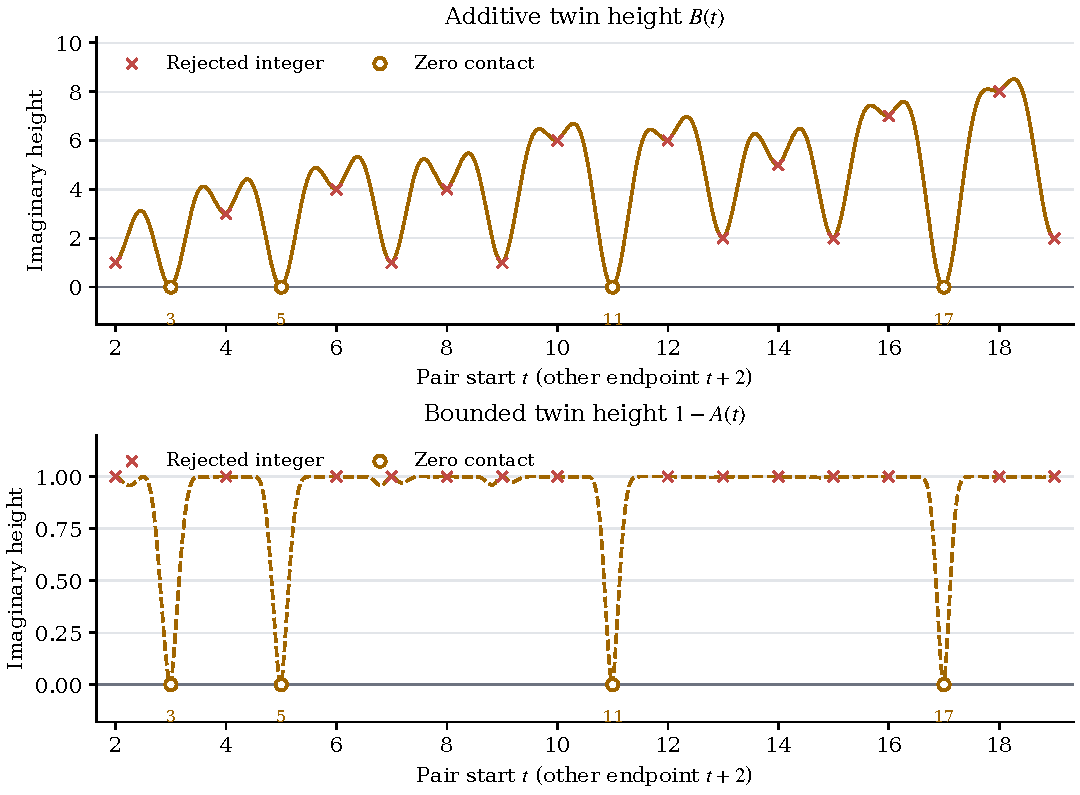
\includegraphics[width=\textwidth]{figures/additive-bounded-twins.pdf}
\caption{Additive and bounded twin heights on pair starts. The curves use
filters through $21$ on $[2,19]$ and have different vertical scales. The
additive height retains divisor counts; the bounded height $1-A(t)$ has
integer values zero or one.}
\label{fig:additive-bounded-twins}
\end{figure}
